\documentclass{article}

\usepackage{url}
\usepackage{microtype}
\usepackage{parskip}
\usepackage[super]{natbib}
\usepackage[a4paper, left=2.5cm, right=2.5cm, top=2.5cm, bottom=2.5cm]{geometry}
\usepackage{longtable,booktabs}
\usepackage{caption}
\usepackage{blindtext}
\usepackage{graphicx}
\usepackage{authblk}
\usepackage{amsmath}
\usepackage{lineno}
\usepackage[toc,page]{appendix}
\usepackage[utf8]{inputenc}
\usepackage{array} %for the tables in appendix
\usepackage{tabularx} %for the tables in appendix

%for algorithms
%\usepackage[ruled,vlined]{algorithm2e}

\usepackage{multicol}
\setlength{\columnsep}{5mm} %column separation

%working title...
\title{Introduction to QGIS (v3.14).\\
	\vspace{0.5cm}
	\large{Schedule and exercises}}
\author[1]{Kerry Pearn (k.pearn@exeter.ac.uk)}

%\affil[1]{\footnotesize University of Exeter Medical School \& NIHR South West Peninsula Applied Research Collaboration (ARC).}
%\affil[1]{\footnotesize Corresponding author: k.pearn@exeter.ac.uk}

\begin{document}
	
\maketitle
	
\section{Schedule} 
	
Today's session: 13:30 - 16:30

\emph{Format:} I will present some QGIS functionality (for up to 20 mins), and then set you an exercise to essentially replicate what I've just demonstrated (for up to 30 mins). During the exercise please use the handout notes (everything you need to complete the exercises are in there) and you will have support on Slack from members of the PenCHORD team and your peers. %Please use us if you need help by posting any questions you have (referencing the numbered point you are working on).

\emph{Itinerary:}
\begin{itemize}
	\item \emph{Section 1:} Introduction to session and datasets 
	\begin{itemize}
		\item slides and data (10 mins)
	\end{itemize}
		
	\item \emph{Section 2:} The QGIS environment, map navigation \& adding your first layer 
	\begin{itemize}
		\item demo (20 mins) \& exercise 1 (15 mins)
	\end{itemize}
	
	\item \emph{Section 3:} Using simple symbology
	\begin{itemize}
		\item demo (20 mins) \& exercise 2 (15 mins)
	\end{itemize}
	
	\item \emph{Section 4:} Point data \& using categorized symbology
	\begin{itemize}
		\item demo (20 mins) \& exercise 3 (20 mins)
	\end{itemize}
	
	\item \emph{Section 5:} Join own data to Shapefile \& using continuous symbology
	\begin{itemize}
		\item demo (20 mins) \& exercise 4 (30 mins)
	\end{itemize}
	
	\item \emph{Section 6:} Print layout
	\begin{itemize}
		\item demo (10 mins) \& exercise if time
	\end{itemize}
	
	\item \emph{Extra material if needed:} Expressions \& dense point data
\end{itemize}

\newpage

\section{Exercise 1.}
\textbf{Aim}: Become familiar with the relationship between the representation of the layer on the map canvas and in the attribute table.\\

Follow these steps. \emph{Use notes from chapters 2 - 5 to help you.}

\begin{enumerate}
	\item Open QGIS
	\item Select \emph{new project} (to get a view with a map canvas)
	\begin{tabular}{@{}c@{}}
\includegraphics[width=3ex]{images/new_project_icon.png}\end{tabular}
	\item Add these toolbars (using menu: View $\rightarrow$ Toolbars)
	\begin{enumerate}
		\item
		Map navigation
		\item
		Data source manager
		\item
		Project
		\item
		Manage layers
		\item
		Attributes
		\item 
		Selection
	\end{enumerate}
	\item Add these panels (using menu: View $\rightarrow$ Panels)
	\begin{enumerate}
		\item
		Browser Panel
		\item
		Layers
		\item
		Layer styling
	\end{enumerate}
	\item Add the world basemap (in coordinate field, in status bar, type "world" and press enter)
	\item Practice map navigation using the world layer. Here's a suggested work sequence to follow:
	\begin{enumerate}
		\item In map canvas, zoom to New Zealand
		\item Create a map view (of New Zealand)
		\item In map canvas, \textit{zoom to layer} for world layer
		\begin{tabular}{@{}c@{}}
\includegraphics[width=3ex]{images/zoom_to_layer_icon.png}\end{tabular}
		\item Close map view (of New Zealand)
		\item In map canvas, zoom to Madagascar
		\item Bookmark this view
		\begin{tabular}{@{}c@{}}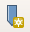
\includegraphics[width=3ex]{images/new_spatial_bookmark.png}\end{tabular}
		\item In map canvas, \textit{zoom to layer} for world layer
		\begin{tabular}{@{}c@{}}
\includegraphics[width=3ex]{images/zoom_to_layer_icon.png}\end{tabular}
	\end{enumerate}
	\item Open attribute table for world layer
	\begin{tabular}{@{}c@{}}
\includegraphics[width=3ex]{images/attribute_table_icon.png}\end{tabular}
	 \& dock attribute table
	 \begin{tabular}{@{}c@{}}
\includegraphics[width=3ex]{images/dock_attribute_table_icon.png}\end{tabular}
	\item Order attribute table alphabetically by Country (feature: NAME)
	\item Select top row of attribute table \& zoom to it on map canvas using \textit{zoom map to selection} icon 
	\begin{tabular}{@{}c@{}}
\includegraphics[width=3ex]{images/zoom_map_to_selection_icon.png}\end{tabular}
	\item \textit{Zoom to layer} for world layer. \begin{tabular}{@{}c@{}}
\includegraphics[width=3ex]{images/zoom_to_layer_icon.png}\end{tabular}
	\item Using \textit{select features} 
	\begin{tabular}{@{}c@{}}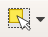
\includegraphics[width=3ex]{images/select_features_icon.png}\end{tabular}
	select the polygon representing Russia within the map canvas (turn yellow)
	\item Using \textit{move selection to top} 
	\begin{tabular}{@{}c@{}}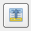
\includegraphics[width=3ex]{images/move_selection_to_top_icon.png}\end{tabular}
	(found in the icons within the attribute table window), bring the details of Russia to the top of the attribute table
	\item Use \textit{Identify tool} 
	\begin{tabular}{@{}c@{}}
\includegraphics[width=3ex]{images/identify_feature_icon.png}\end{tabular}
	and click on the polygon representing Russia to view the same details stored in the attribute table in the \textit{Identify Results} panel.
	\item To remove identify function, either select another icon, e.g. the \textit{pan map} icon 
	\begin{tabular}{@{}c@{}}
\includegraphics[width=3ex]{images/pan_map_icon.png}\end{tabular}
	, or click the sea.
	\item \textit{zoom to layer} for world layer
	\begin{tabular}{@{}c@{}}
\includegraphics[width=3ex]{images/zoom_to_layer_icon.png}\end{tabular}
	\item Save project. Close QGIS. Reopen QGIS \& your project.
\end{enumerate}

\textbf{Result}: At the end this exercise your QGIS project should show the useful toolboxes and panels, a single layer (world) listed in the layers panel, the world layer in full zoom on the map canvas, and the world layer's attribute table docked to the bottom of the map canvas.

\section{Exercise 2.}
\textbf{Aim}: Extract some features from the world layer, and save them as a new shapefile. Become familiar with the \textit{Layers Styling} panel in order to change the appearance of the layer using simple symbology.\\

Follow these steps. \emph{Use notes from chapter 6 - 8 to help you.}
\begin{enumerate}
	\item Change the project projection to EPSG: 32630 (see chapter 6).
	\item From the world layer, select polygons for UK. These are now your "selected features" (see chapter 7).
	\item Export selected features to new shapefile called "UK.shp" (see chapter 7).
	\item Play with the order of the two layers in the layers panel (world and UK). Toggle between having both/one/none selected (please end with the UK being the only one selected, and zoom to this layer)
	\item Customise the simple symbology for the UK shapefile (follow Chapter 8). 
\end{enumerate}

\textbf{Result}: At the end this exercise your QGIS project should show the UK as land and coast

\section{Exercise 3}

\textbf{Aim}: Add point data from a delimited text file (.csv) and style the points using categorised symbology\\
 
\textbf{Exercise 3A}: Add your Police HQ point data and style each point to represent whether the site is also a Fire and Rescue HQ. Follow these steps, and \emph{use notes from chapter 11 to help you.}
\begin{enumerate}
	\item Add delimited file
	\begin{tabular}{@{}c@{}}
\includegraphics[width=3ex]{images/add_delimited_text_layer_icon.png}\end{tabular}
 	to project: $headquarters.csv$

	Within the \textit{Data Source Manager / Delimited text} window, choose these settings:\\
	\textbf{File name:} Navigate to the csv file: $headquarters.csv$\\
	\textbf{Layer name} (what appears in the \textit{Layers Panel}, so choose something meaningful): street\_crime\\
	\textbf{File Format}: CSV (comma separated values)\\
	\textbf{Geometry definition} $\rightarrow$ Point coordinates $\rightarrow$  
	\textbf{x field} = Longitude \& \textbf{y field} = Latitude\\
	\textbf{Coordinate system}: EPSG4326 – WGS 84 (leave as default)\\
	\textbf{Add}.

	\item Use the field "Fire\_Rescue\_HQ\_site" (a boolean to represent whether the feature is also a Fire and Rescue HQ) to format the points to show this information.
	
	In the \textit{Layers Styling} panel:\\
	Select \textit{headquarters}\\
	Select \textit{Categorized}\\
	\textbf{Column}: Fire\_Rescue\_HQ\_site.\\
	\textbf{Classify}
	\item Choose the style for each symbol
	\item Set legend text to \textit{"Police HQ"} and \textit{"Police \& Fire Rescue HQ"}.
\end{enumerate}

\newpage

\textbf{Exercise 3B}: Add a label to each point to state the site's location (using field "Head quarters"). Follow these steps, and \emph{use notes from chapter 12 to help you.}

\begin{enumerate}
	\item In the \textit{Layer Styling} panel select the layer \textit{headquarters}.
	\item Click the \textit{Labels} icon on the LHS of the \textit{Layer styling} panel.
	\item Select “Single labels”
	\item Value: Head quarters
	\item Experiment with changing the settings under the various style tabs to create your label visualisation.
	\item If time, follow the instructions in the notes for section 12.3 to \textit{Put a number in a point}

\end{enumerate}

\textbf{Result}: At the end this exercise your QGIS project should show the UK basemap, with 5 points for the locations of the Police headquarters, points styled based on site type, and a label showing the site name. 

\section{Exercise 4}

\textbf{Aim}: Become familiar with joining your own data (.csv file) to a corresponding shapefile in order to visualise your data. Use continuous symbology to style the layer.\\

\textbf{Exercise 4A}: Add delimited text file, add shapefile and create a table join \emph{Use notes from chapter 13 \& 14 to help you.}
\begin{enumerate}
	\item Add vector layer
		\begin{tabular}{@{}c@{}}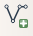
\includegraphics[width=3ex]{images/add_vector_layer_icon.png}\end{tabular}
		 to your QGIS project: $LSOA\_2011\_sw5forces\_BGC\_V2.shp$
	\item Open the attribute table \& dock. If have time, you can practice what you've learnt on this shapefile, such as:
\begin{enumerate}
		\item Move between selecting features on the map canvas (select feature tool
		\begin{tabular}{@{}c@{}}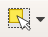
\includegraphics[width=3ex]{images/select_features_icon.png}\end{tabular}		
		), and identifying them in the attribute table (move selected rows to top of table
		\begin{tabular}{@{}c@{}}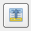
\includegraphics[width=3ex]{images/move_selection_to_top_icon.png}\end{tabular}). 
		\item Move between selecting features in the attribute table, and identifying them in the map canvas (zoom to selected features
		\begin{tabular}{@{}c@{}}
\includegraphics[width=3ex]{images/zoom_map_to_selection_icon.png}\end{tabular}). 
		\item Save selected feature as new feature layer (try creating a shapefile for just the Exeter features)
		\item Use Identify feature tool
		\begin{tabular}{@{}c@{}}
\includegraphics[width=3ex]{images/identify_feature_icon.png}\end{tabular}. 
		\item Zoom to UK layer and deselect features
		\begin{tabular}{@{}c@{}}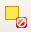
\includegraphics[width=3ex]{images/deselect_features_icon.png}\end{tabular}. 
	\end{enumerate}
	\item Add this delimited text layer
	\begin{tabular}{@{}c@{}}
\includegraphics[width=3ex]{images/add_delimited_text_layer_icon.png}\end{tabular}
	: $sw\_5forces\_street\_by\_lsoa.csv$.
	\item Open the attribute table for this layer. Identify the common column within each of the two layers about to join.
	\item Table join: Join data from csv file to shapefile (follow section 14.3 in the notes).	
\end{enumerate}


\textbf{Exercise 4B}: Use graduated symbology to style your layer \emph{Use notes from chapter 15 to help you.}
\begin{enumerate}
	\item Using the information covered in chapter 15, choose two columns from the street crime dataset, and style them using graduated symbology. Whilst doing this please also: 
	\begin{enumerate}
		\item Edit the text to be used in the legend (usually involves removing the unnecessary decimals)
		\item Have a separate layer displaying the visualisation for each column (duplicate the layer)
		\item Rename each layer
		\item Within the \textit{Layers} panel, put these two layers in a group with the property \textit{Mutually Exclusive} (see chapter 10).
	\end{enumerate}
\end{enumerate}

\textbf{Result}: At the end this exercise your QGIS project should show LSOA crime data for the SW, styled to represent a data field, together with a UK basemap \& the 5 locations of the Police headquarters. 

\end{document}
